\documentclass[border=0pt]{standalone}
\usepackage{pgfplots}
\pgfplotsset{width=\linewidth,compat=1.8}
\usepackage{pgfplotstable}
\usepackage{amsmath}
\begin{document}

% \pgfplotsset{every tick label/.append style={font=\boldmath\huge}}

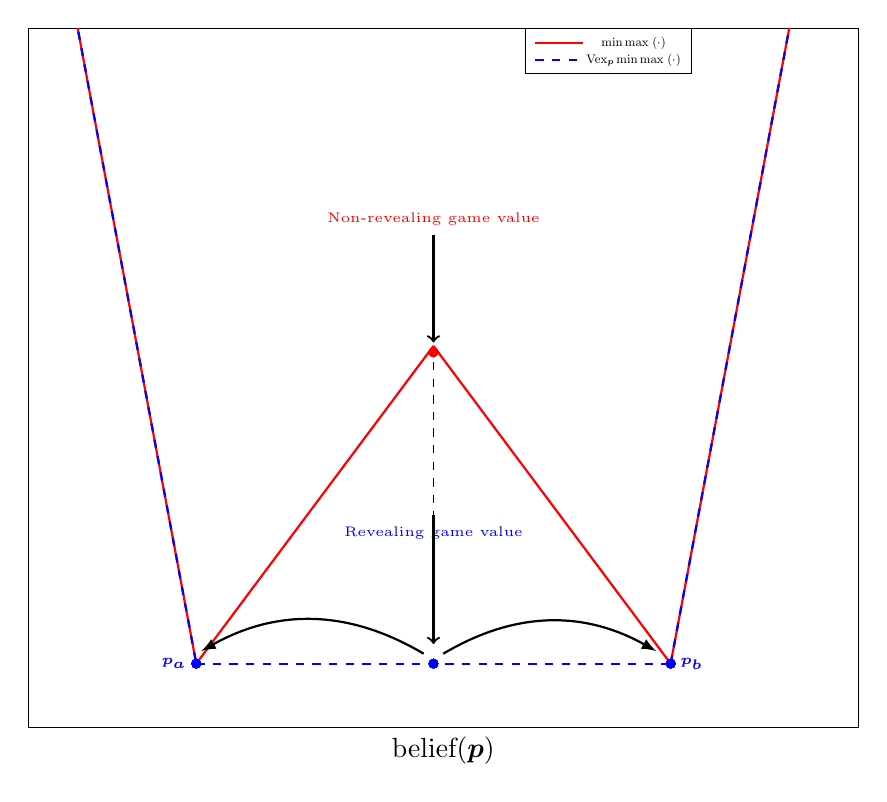
\begin{tikzpicture}
% \tikzstyle{every node}=[font=\tiny]
\begin{axis}[ymax=1, xlabel= belief$(\boldsymbol{p})$, ticks=none, 
    legend entries={\small $\min \max\;(\cdot)$, \small $\text{Vex}_{\boldsymbol{p}} \min \max\;(\cdot)$},
        legend style={nodes={scale=0.5}, style={at={(0.8, 1)}}}]
    \addlegendimage{red, thick}
    \addlegendimage{blue, thick, dashed}
    \addplot[color=red, domain=0:1, thick]{-4*(x-1)};
    \addplot[color=red, domain=1:1.5, thick]{1*(x-1)};
    \addplot[color=red, domain=1.5:2, thick]{-1*(x-1) + 1};
    \addplot[color=red, domain=2:3, thick]{4*(x-1)-4};
    \addplot[color=blue, dashed, domain=0:1, thick]{-4*(x-1)};
    \addplot[color=blue, dashed, domain=2:3, thick]{4*(x-1)-4};
    \addplot[color=blue, dashed, domain=1:2, thick]{0};
    \addplot [mark=*, color=blue, mark size=1.5pt](1, 0) node[left] {\tiny $\boldsymbol{p}_{\boldsymbol{a}}$};
    \node at (99, 2) (A) {};
    \addplot [mark=*, color=blue, mark size=1.5pt](2, 0) node[right] {\tiny $\boldsymbol{p}_{\boldsymbol{b}}$};
    \node at (199, 2) (B) {};
    \addplot [mark=*, color=red, mark size=1.5pt](1.5, 0.49) node (N) {};
    \node [red] at (150, 70) (C2)  {\tiny Non-revealing game value};
    \draw[->, thick] (C2) -- (N);
    \addplot [mark=*, color=blue, mark size=1.5pt](1.5, 0) node[above] (C) {};
    \draw [decorate,decoration={show path construction,
    lineto code={\draw[-latex, thick] (\tikzinputsegmentfirst) to[bend right](\tikzinputsegmentlast); }}]
    (C) -> (A);
    \draw [decorate,decoration={show path construction,
    lineto code={\draw[-latex, thick] (\tikzinputsegmentfirst) to[bend left](\tikzinputsegmentlast); }}]
    (C) -> (B);
    \node [blue, above] at (150, 18) (D) {\tiny Revealing game value};
    \node  at (150, 25) (C1) {};
    \draw[->, thick] (C1) -- (C);
    \draw[dashed] (N) -- (C);
\end{axis}
\end{tikzpicture}
\end{document}